% - add recovered state
% - add probability to become recovered
In order for us to add the recovered class and visualize them properly, we had to change the following files:
\begin{itemize}
    \item \textbf{AttributesSIRG:} 
    \begin{itemize}
        \item New method \texttt{getRecoveredfixedRate()} which returns the new value of \texttt{recoveredfixedRate} set arbitrarily at 0.2 (the probability for an INFECTED individual to become recovered/removed).
    \end{itemize}

    \item \textbf{SIRType:} 
    \begin{itemize}
        \item Added the type \texttt{ID\_REMOVED} for the removed group.
    \end{itemize}

    \item \textbf{SIRGroupModel:} 
    \begin{itemize}
        \item To include the removed class, we had to change the method \texttt{getFreeGroupId()} to include the new group of recovered individuals. Figure \ref{fig:SIRGroupModel_code_change} shows the change in the function. It was a simple fix to include the recovered class with a similar logic as the infected group. We also had to change the \texttt{Update function} to add infected individuals to the recovered class based on a certain probability. 
        \begin{figure}[h]
            \centering
            \begin{subfigure}[b]{0.5\textwidth}
                 \centering
                 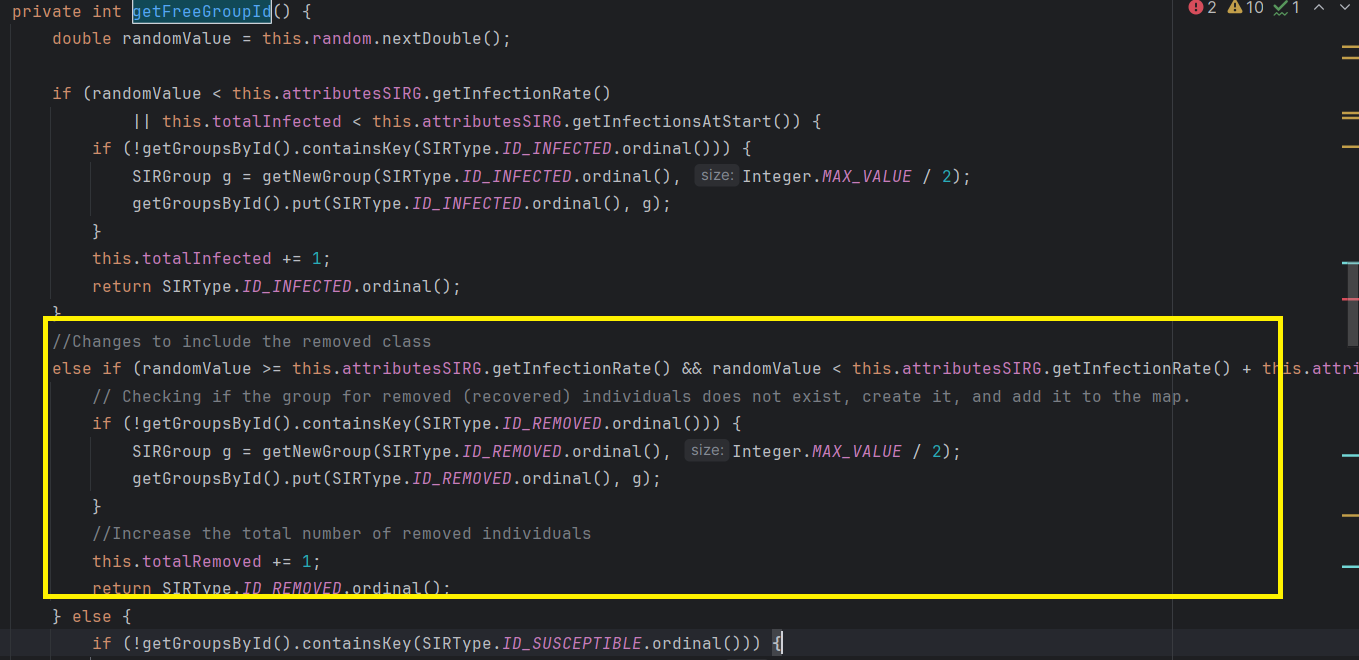
\includegraphics[width=\textwidth]{images/removedClassCode.png}
                \caption{getFreeGroupId() changes in SIRGroupModel}
                \label{task5CodeChangea}
             \end{subfigure}
            \begin{subfigure}[b]{0.5\textwidth}
                 \centering
                 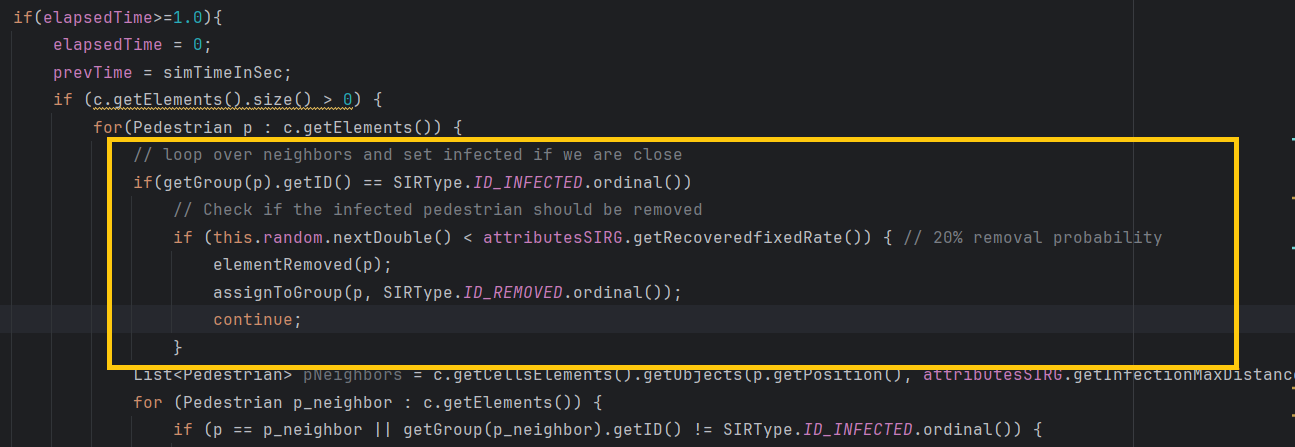
\includegraphics[width=\textwidth]{images/removedClassCOdeChange2.png}
                \caption{Changes in update method of SIRGroupModel}
                \label{fig: task5CodeChangeb}
             \end{subfigure}
            \caption{Code changes in SIRGroupModel to include recovered class.}
            \label{fig:SIRGroupModel_code_change}
        \end{figure}
    \end{itemize}

    \item \textbf{utils.py:} 
    \begin{itemize}
        \item We changed the function \texttt{create\_folder\_data\_scatter(folder)} in the provided SIRVisualization utils file (\texttt{DASH/plotly} visualizer) to allow us to visualize the recovered class.
    \end{itemize}
\end{itemize}




% - visualisation
% - tests

To test our implementation we conducted multiple experiments on our modified software. The first test we conduct is the same as in figure \ref{fig:task4.5_1} from task 4, with the only difference that pedestrians now can recover after being infected. The end frame for task 5 can therefore look like the ones in figure \ref{fig: 51ad}, with different distributions of blue and green dots for susceptible and recovered pedestrians. \\
Figure \ref{fig: 5ad} shows a comparison of different infection and recovery rates. In subfigure \ref{fig: 5a}, a low infection rate (0.05) and a high recovery rate (0.2) are used. Only 202 pedestrians become infected over time and a constant value is established after 70 time steps. In subfigure \ref{fig: 5b}, the infection rate is doubled (0.1), while the recovery rate stays the same (0.2). In comparison, a drastic difference can be seen: the susceptible and removed lines almost close the gap in between with a total number of 473 infected and later removed pedestrians after 60 time steps. Subfigure \ref{fig: 5c} changes the recovery parameter to 0.1, and the infection parameter stays at 0.1. Here, the initial spike in infections is much higher, and a total of 790 infections after 86 time steps. Finally, subfigure \ref{fig: 5d} is created with an infection rate of 0.05 and a recovery rate of 0.1. It looks the closest to the second parameter settings, however, the lines intersect, and the infections reach a total of 630 after 103 time steps.

\begin{figure}[H]
 \centering
 \begin{subfigure}[b]{0.4\textwidth}
     \centering
     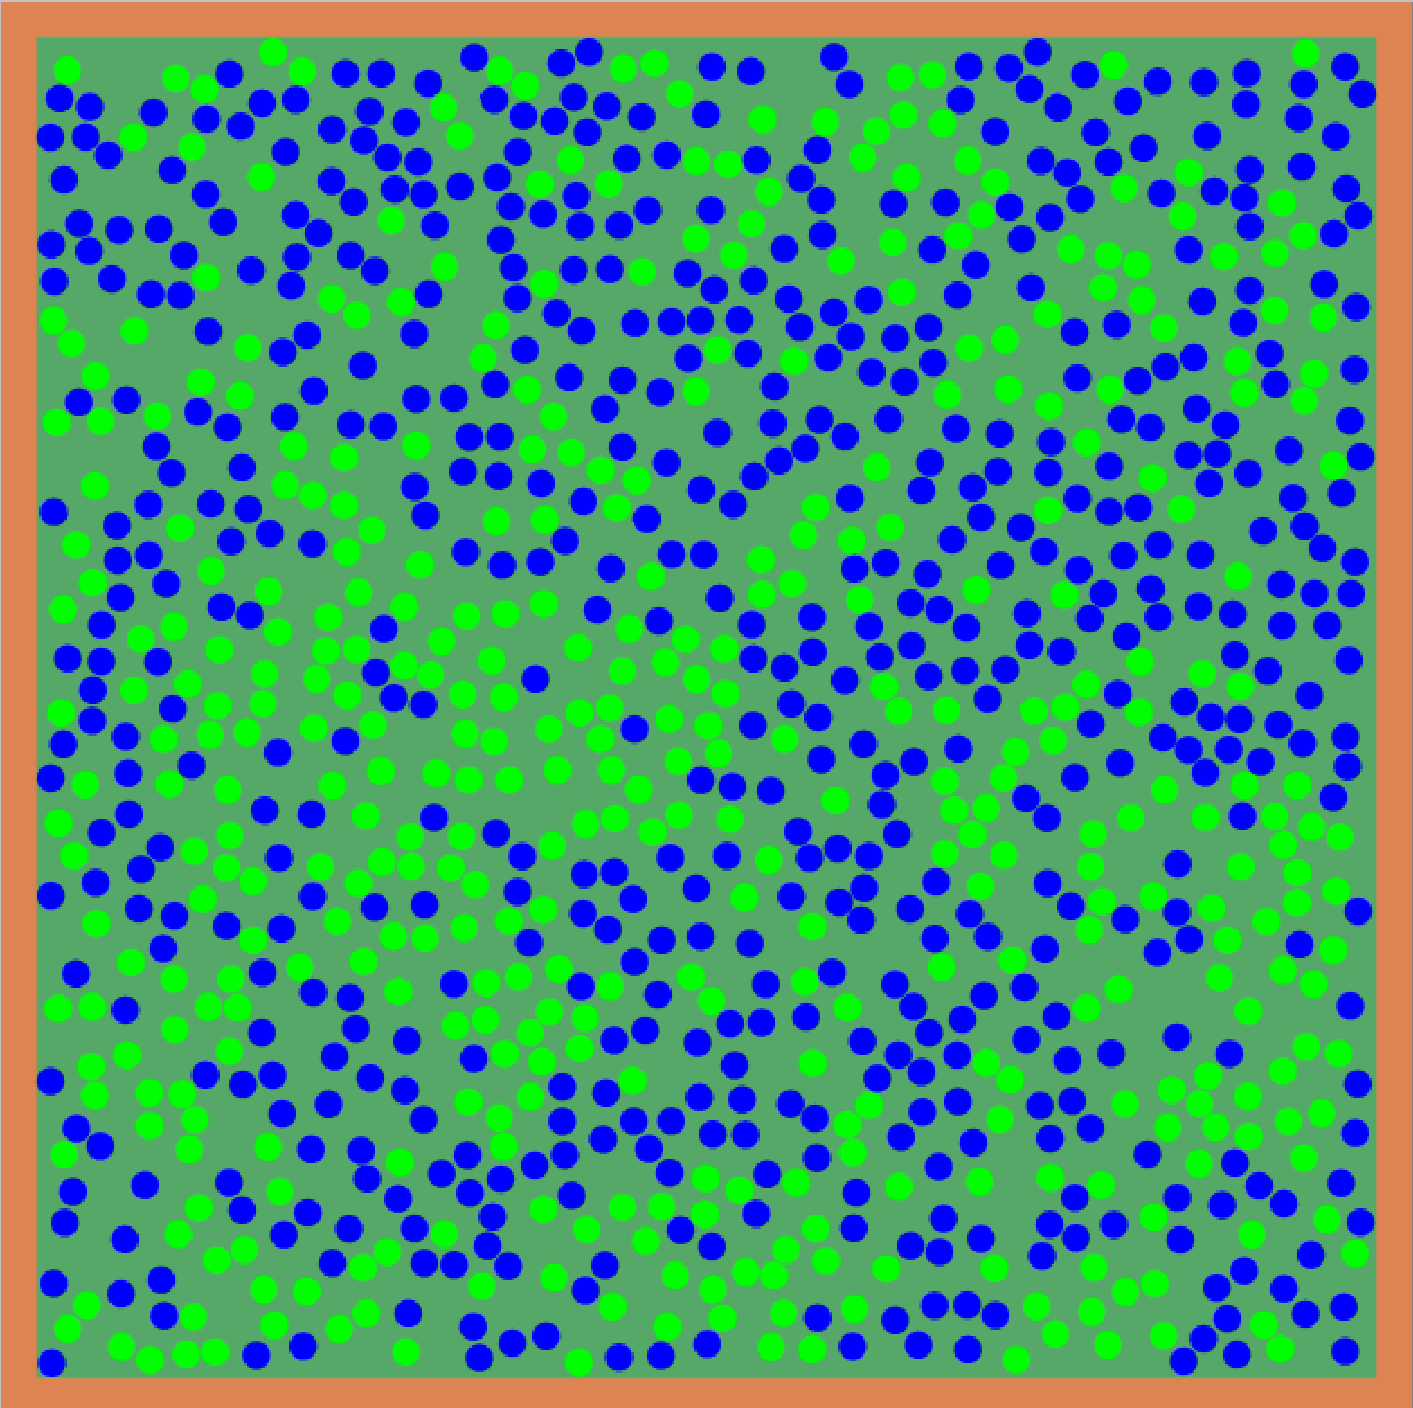
\includegraphics[width=0.8\textwidth]{images/2-51a.png}
    \caption{I: 0.05 - R: 0.2}
    \label{fig: 51a}
 \end{subfigure}
 \begin{subfigure}[b]{0.4\textwidth}
      \centering
     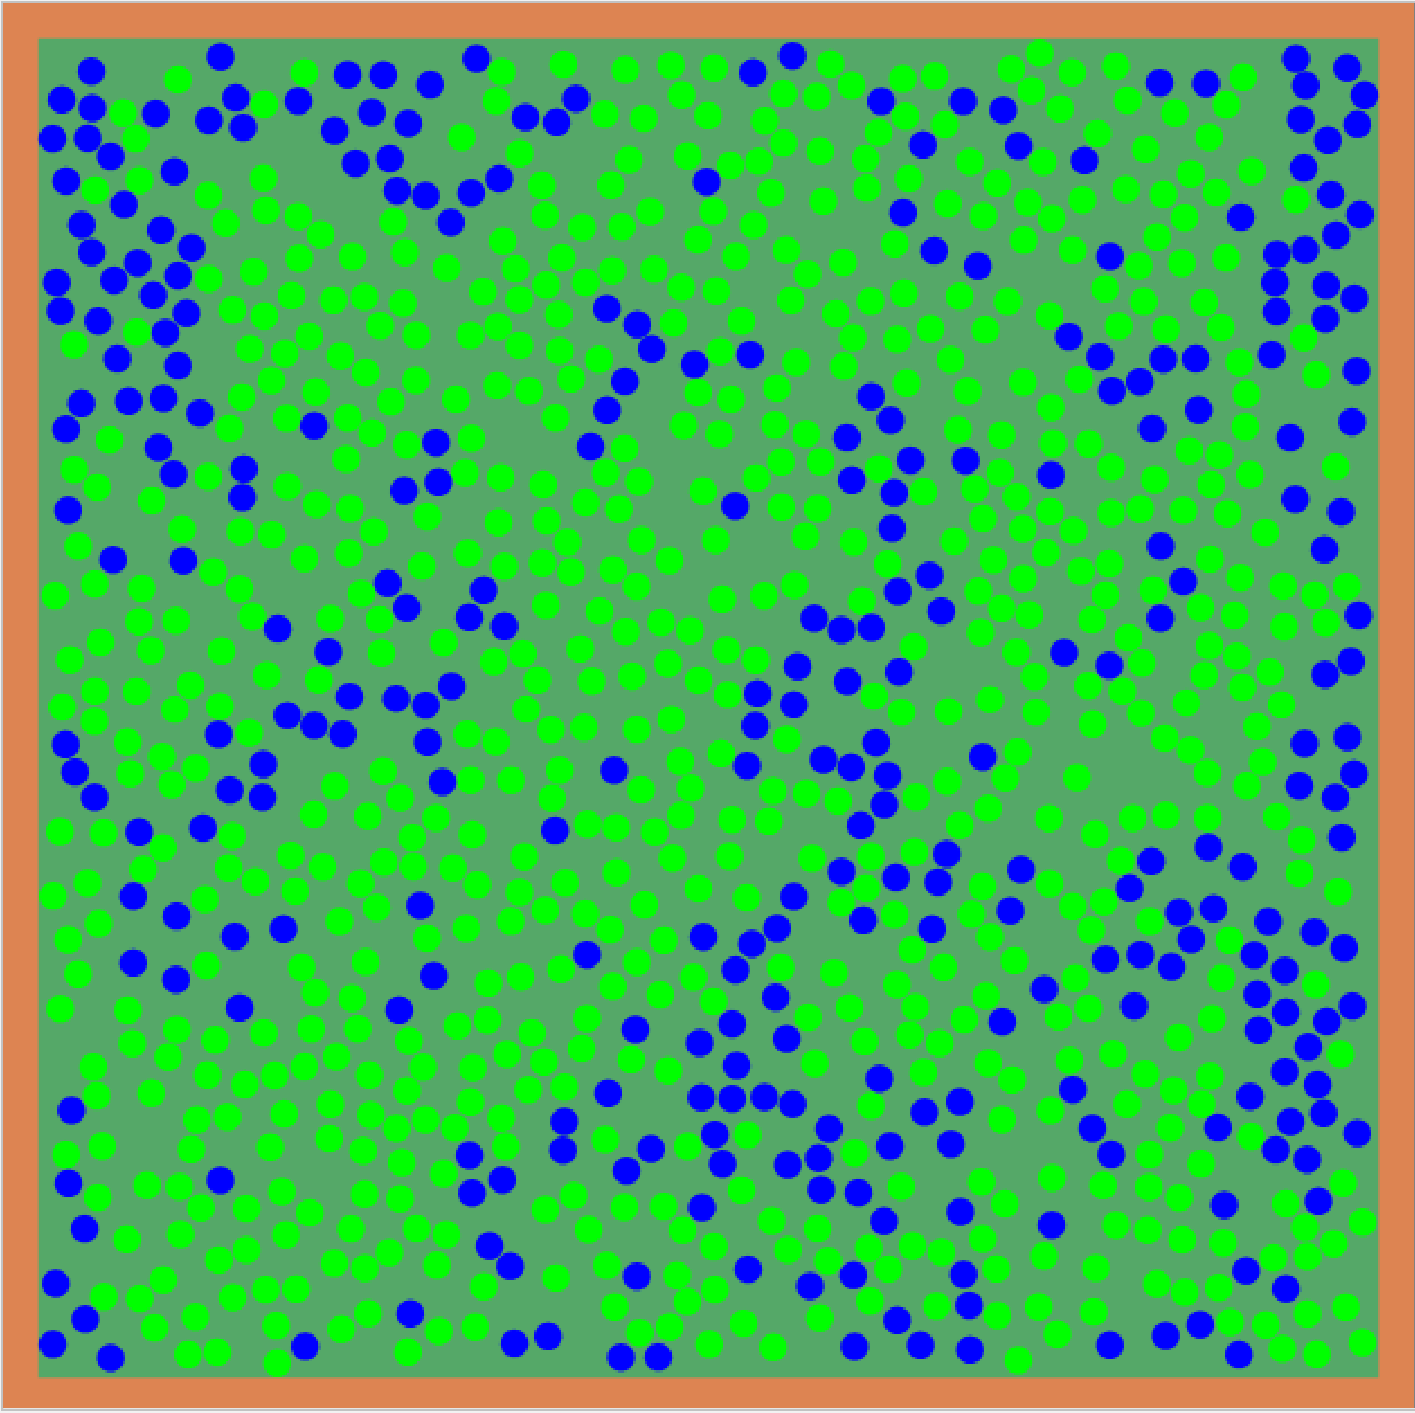
\includegraphics[width=0.8\textwidth]{images/2-51b.png}
     \caption{I: 0.1 - R: 0.2}
     \label{fig: 51b}
 \end{subfigure}
 \begin{subfigure}[b]{0.4\textwidth}
      \centering
     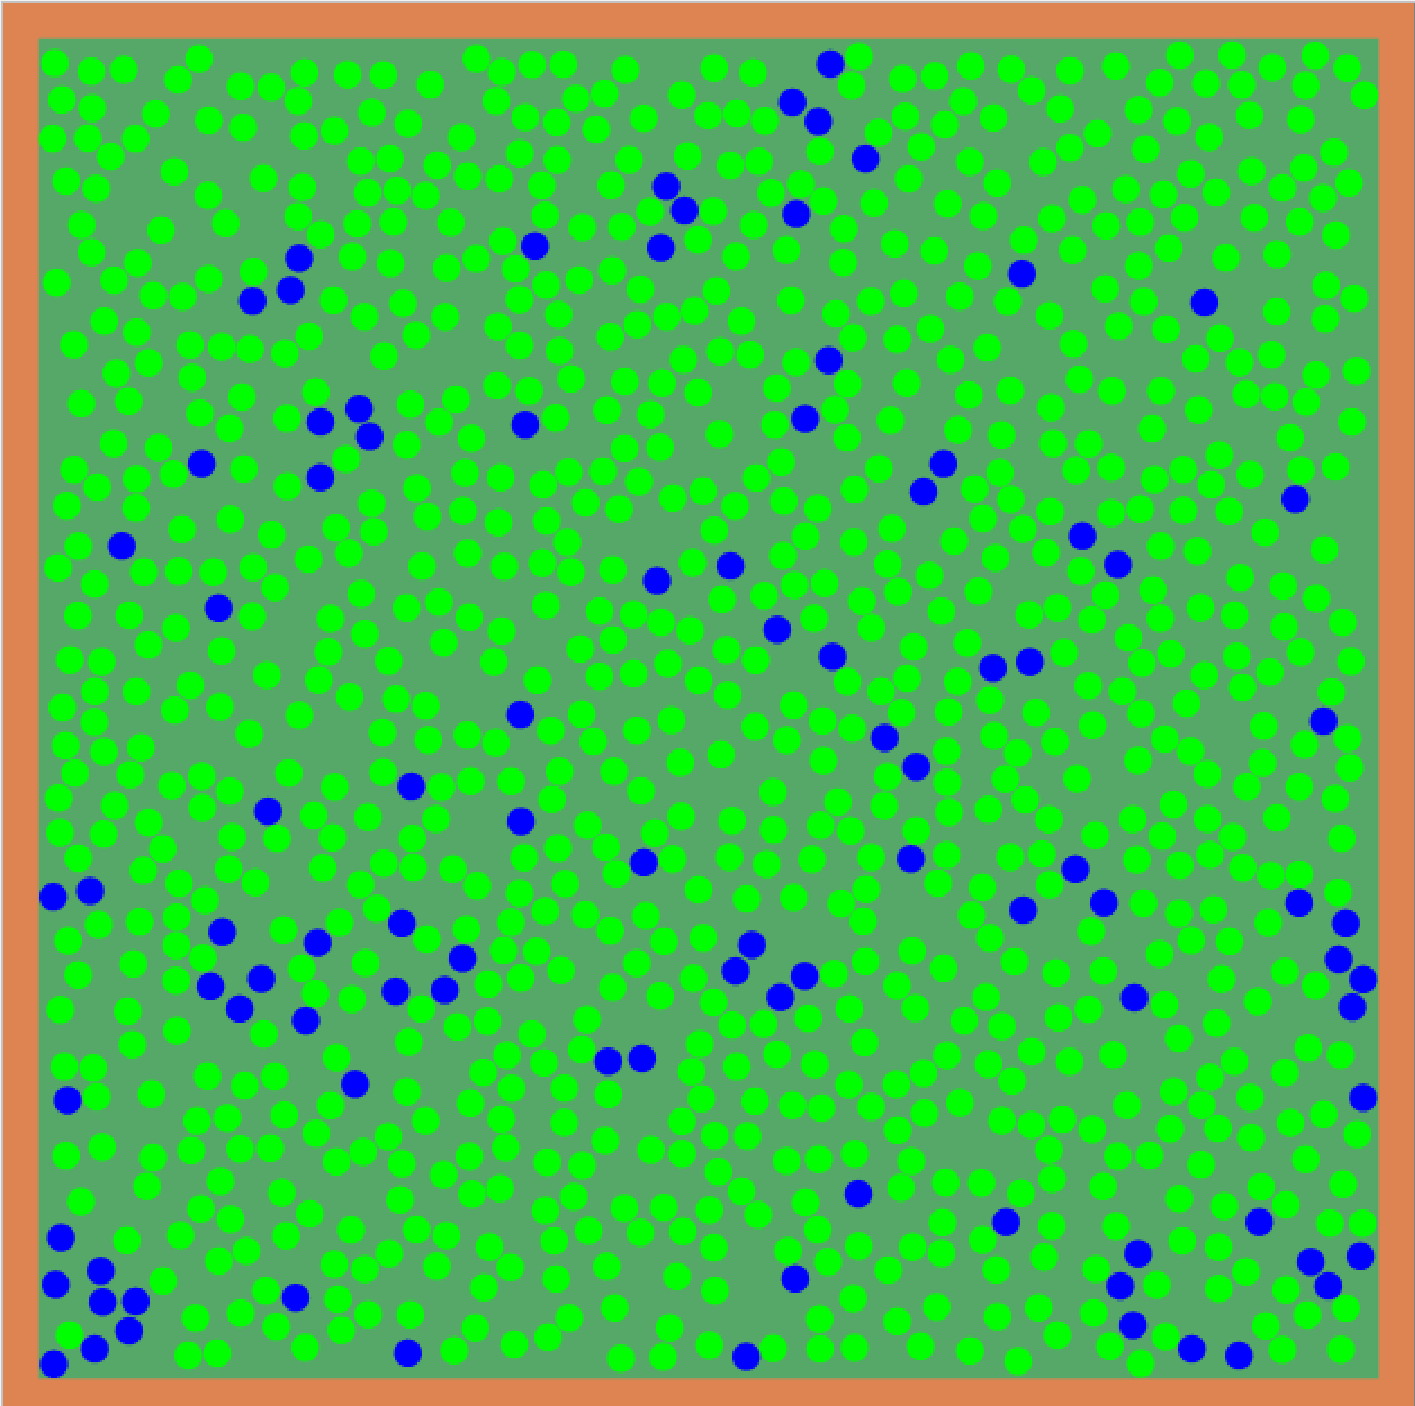
\includegraphics[width=0.8\textwidth]{images/2-51c.png}
     \caption{I: 0.1 - R: 0.1}
     \label{fig: 51c}
 \end{subfigure}
 \begin{subfigure}[b]{0.4\textwidth}
      \centering
     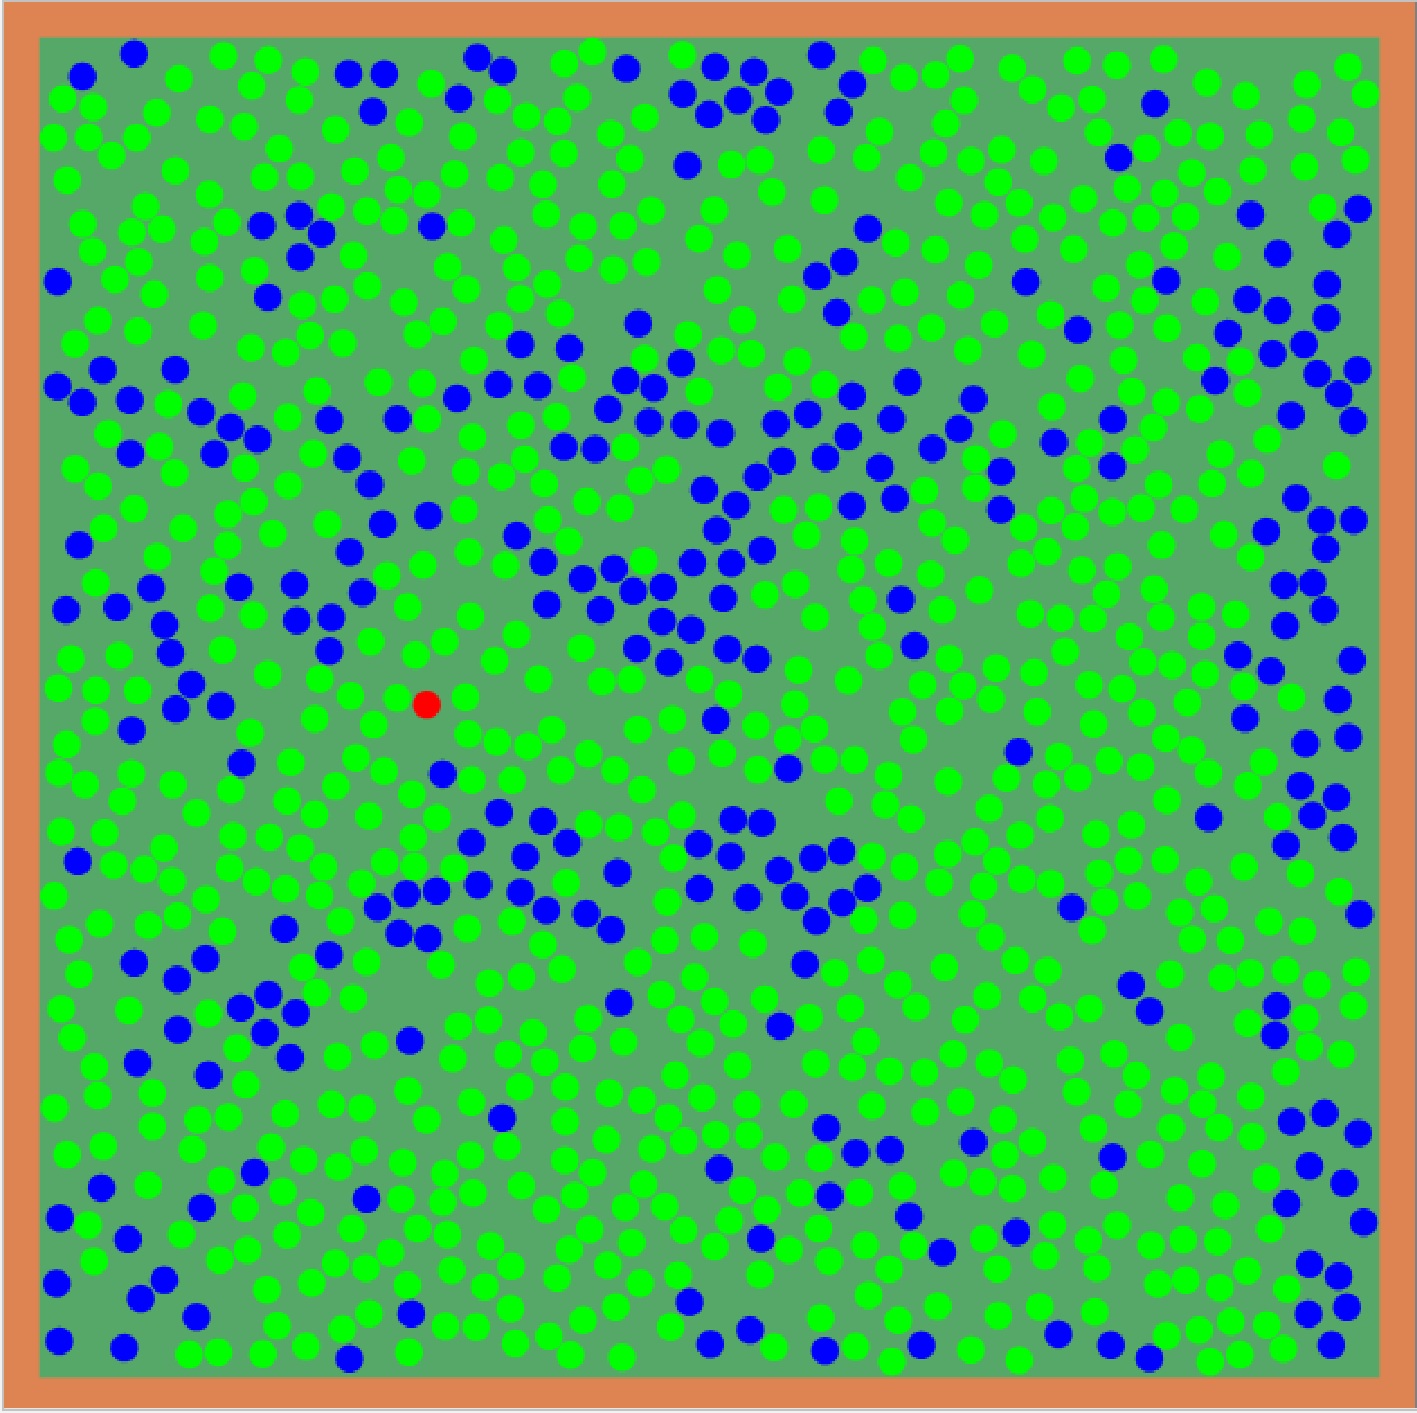
\includegraphics[width=0.8\textwidth]{images/2-51d.png}
     \caption{I: 0.05 - R: 0.1}
     \label{fig: 51d}
 \end{subfigure}
 \caption{Final simulation picture for different infection (I) and recovery (R) rates}
 \label{fig: 51ad}
\end{figure}

\begin{figure}[H]
 \centering
 \begin{subfigure}[b]{\textwidth}
     \centering
     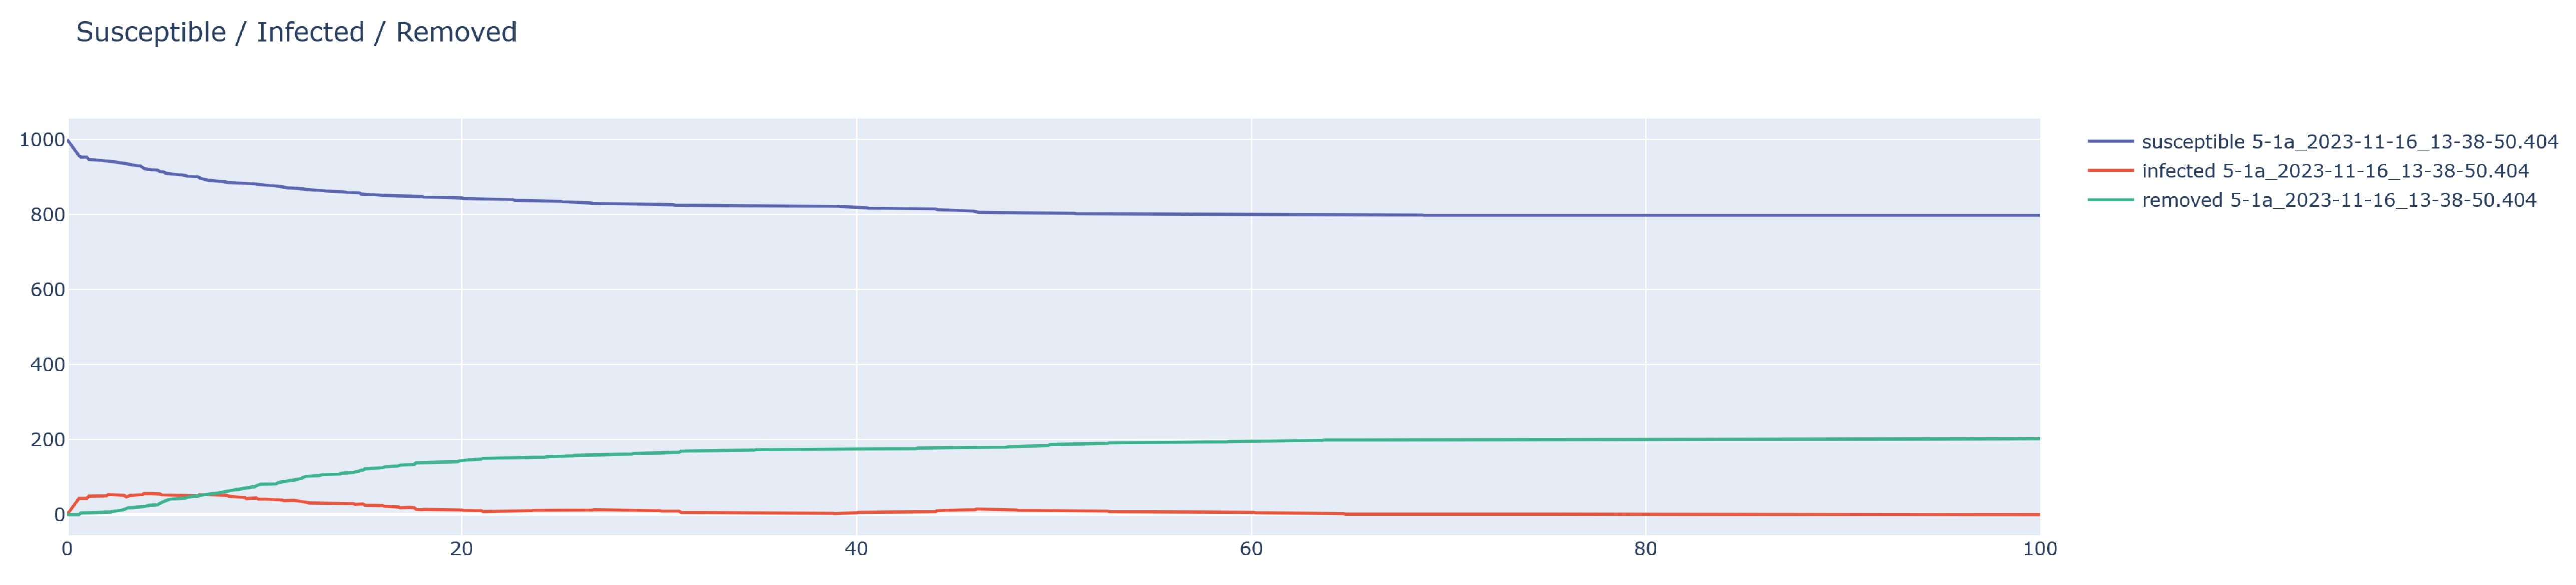
\includegraphics[width=\textwidth]{images/2-5a.png}
    \caption{I: 0.05 - R: 0.2}
    \label{fig: 5a}
 \end{subfigure}
 \begin{subfigure}[b]{\textwidth}
      \centering
     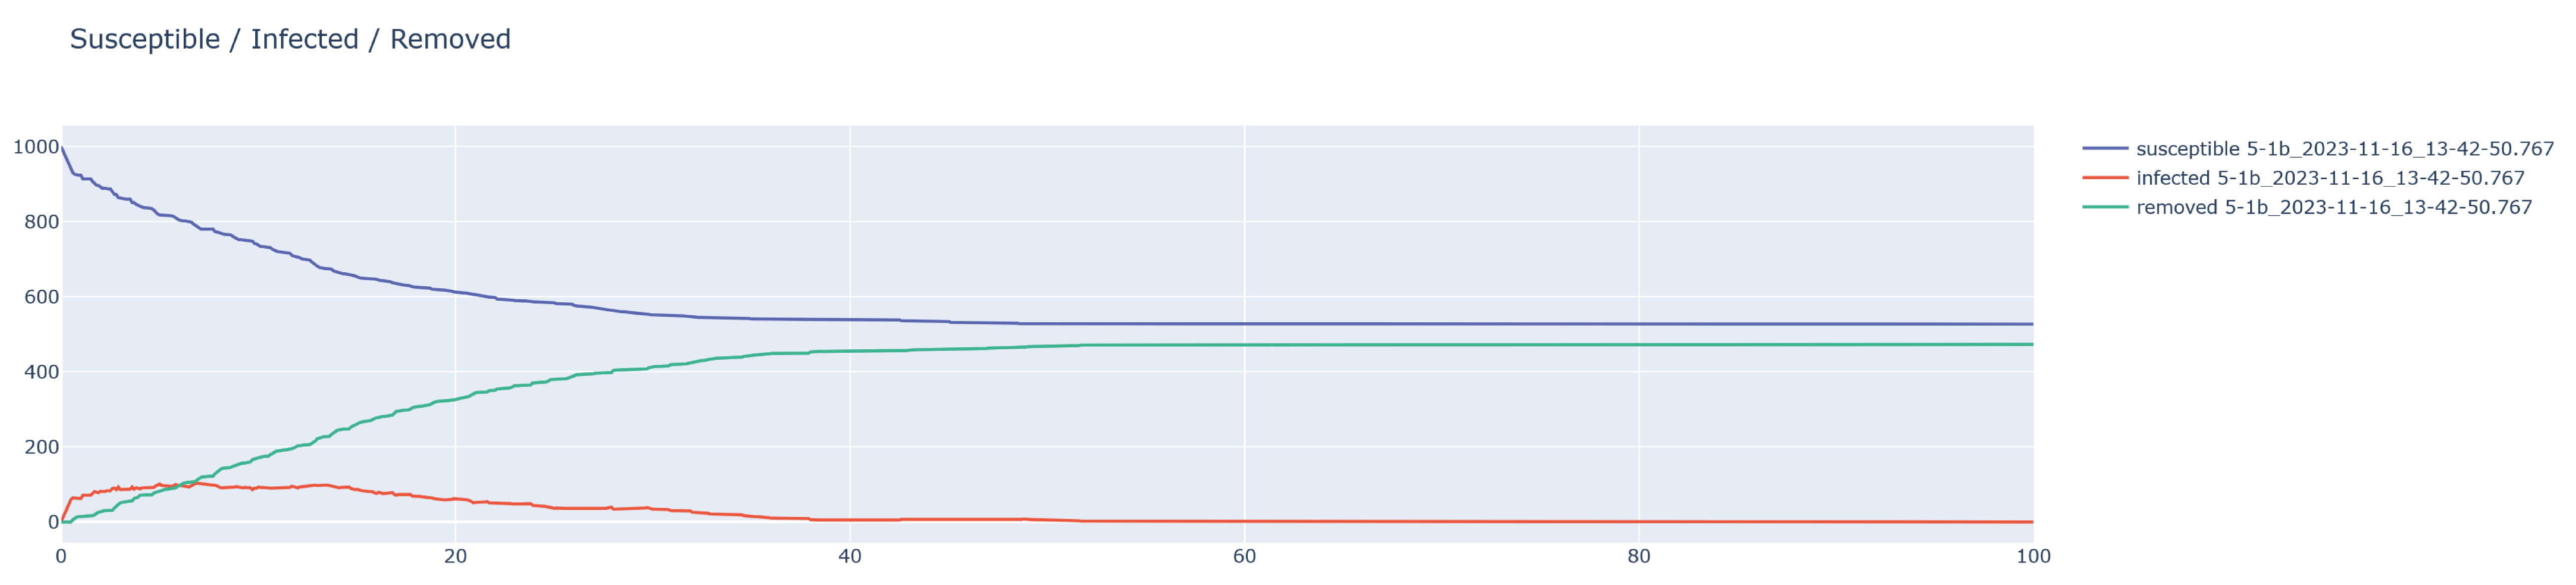
\includegraphics[width=\textwidth]{images/2-5b.png}
     \caption{I: 0.1 - R: 0.2}
     \label{fig: 5b}
 \end{subfigure}
 \begin{subfigure}[b]{\textwidth}
      \centering
     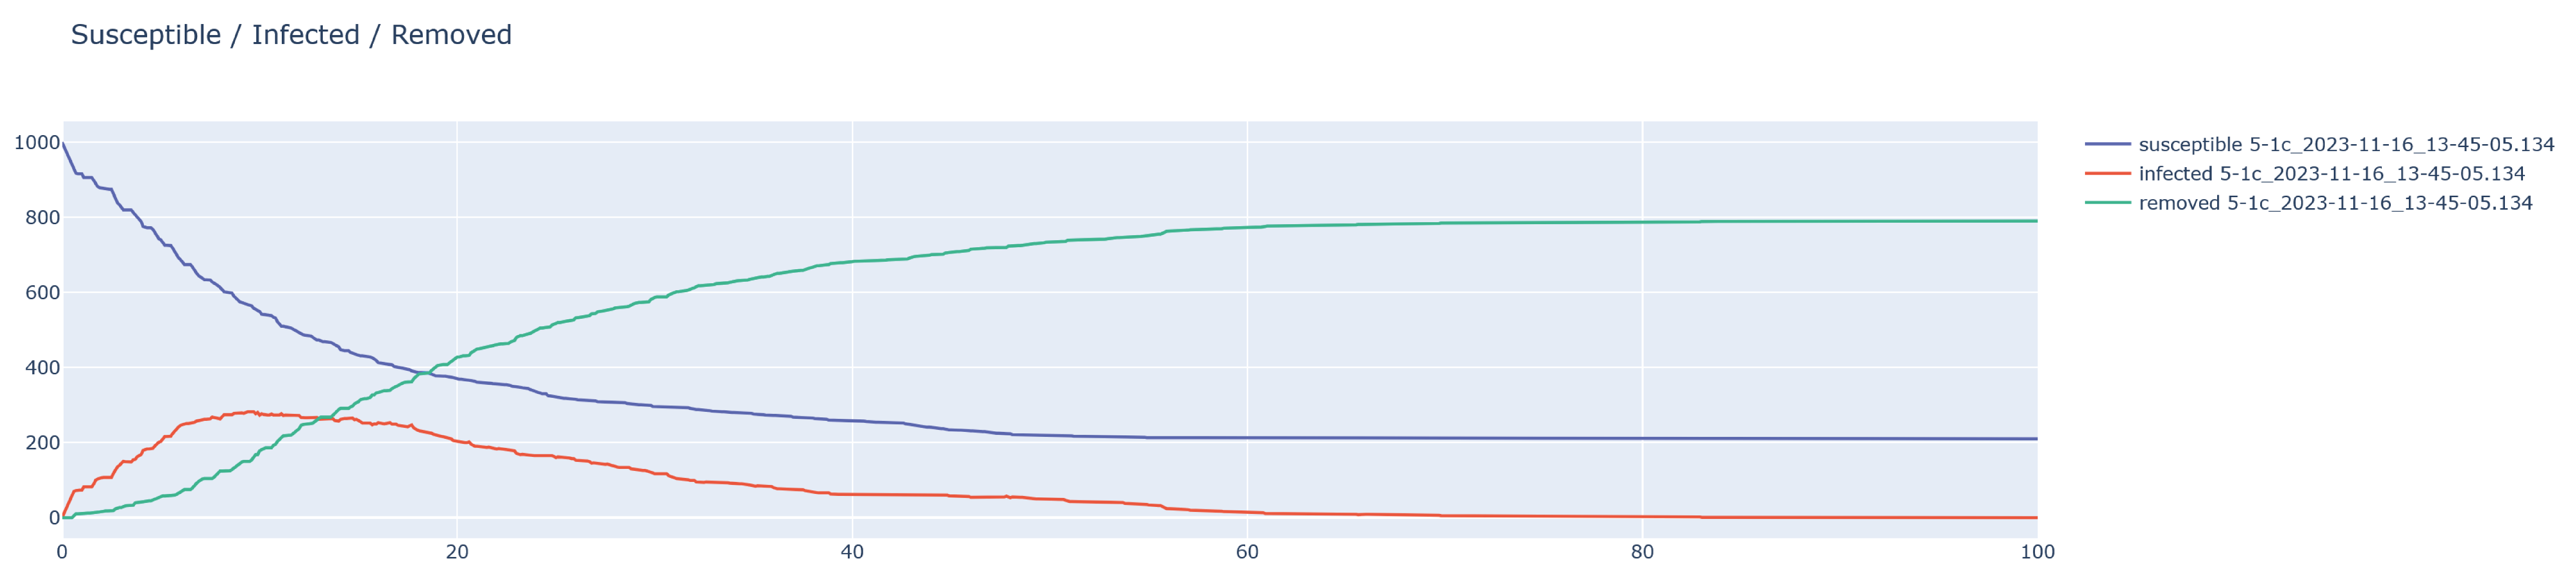
\includegraphics[width=\textwidth]{images/2-5c.png}
     \caption{I: 0.1 - R: 0.1}
     \label{fig: 5c}
 \end{subfigure}
 \begin{subfigure}[b]{\textwidth}
      \centering
     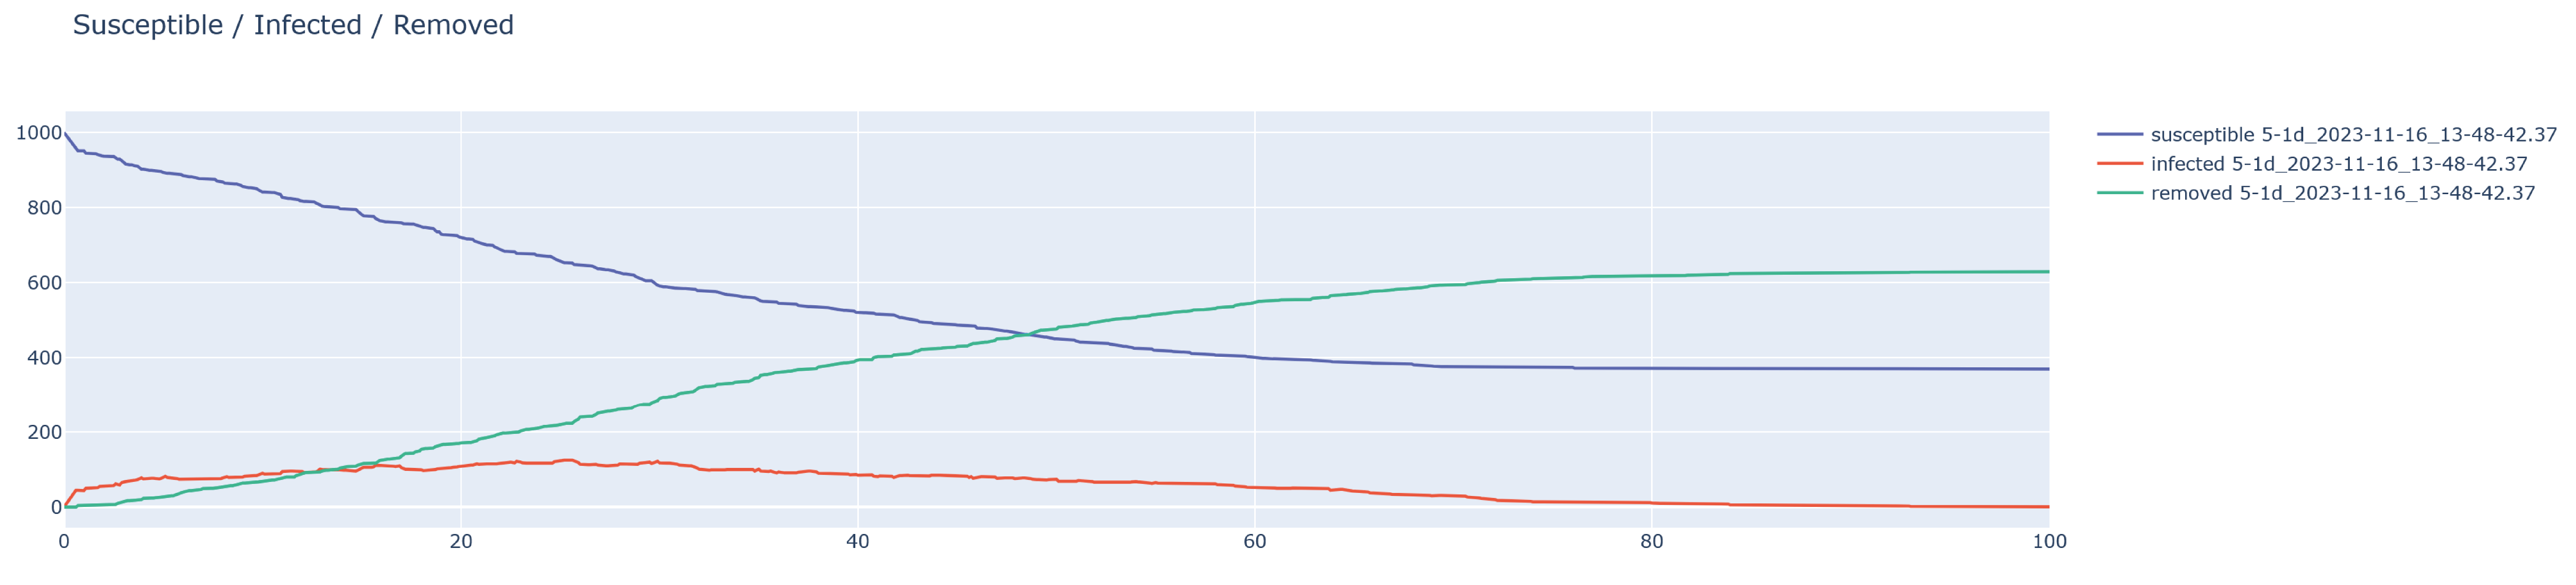
\includegraphics[width=\textwidth]{images/2-5d.png}
     \caption{I: 0.05 - R: 0.1}
     \label{fig: 5d}
 \end{subfigure}
 \caption{Comparison of different infection (I) and recovery (R) rates}
 \label{fig: 5ad}
\end{figure}

\textit{\textbf{Supermarket simulation}}

To create a fairly realistic scenario of a supermarket, we took inspiration from the supermarket model available on \href{https://www.smartdraw.com/store-layout/examples/grocery-store-layout/}{smartdraw}. To comply with the requirement of having a supermarket of at least 30x30m, however, all dimensions have been roughly doubled compared to the previous model, which may affect the realism of the simulation.

\begin{figure}[H]
    \begin{subfigure}[b]{0.49\textwidth}
        \centering
        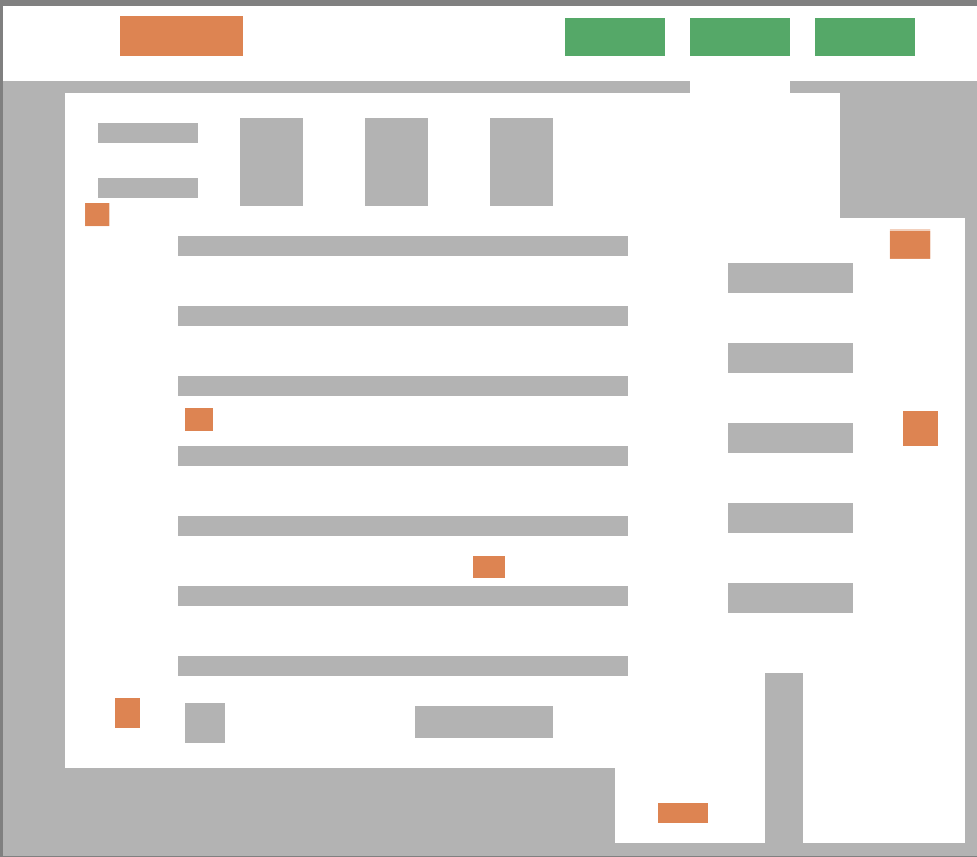
\includegraphics[width=\textwidth]{images/supermarket_design.png}
        \caption{Supermarket model}
        \label{fig:supermarket_a}
    \end{subfigure}
    \hfill
    \begin{subfigure}[b]{0.49\textwidth}
        \centering
        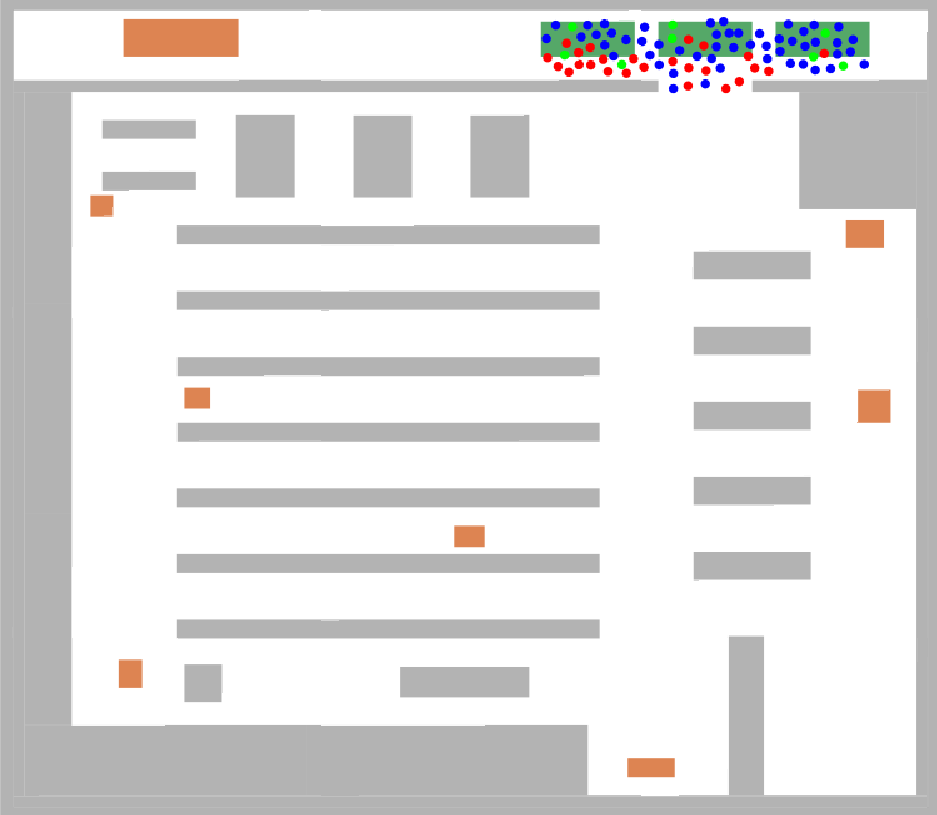
\includegraphics[width=\textwidth]{images/task5_shoppingbegin.png}
        \caption{Pedestrians enter the supermarket}
        \label{fig:supermarket_b}
    \end{subfigure}

    \begin{subfigure}[b]{0.49\textwidth}
        \centering
        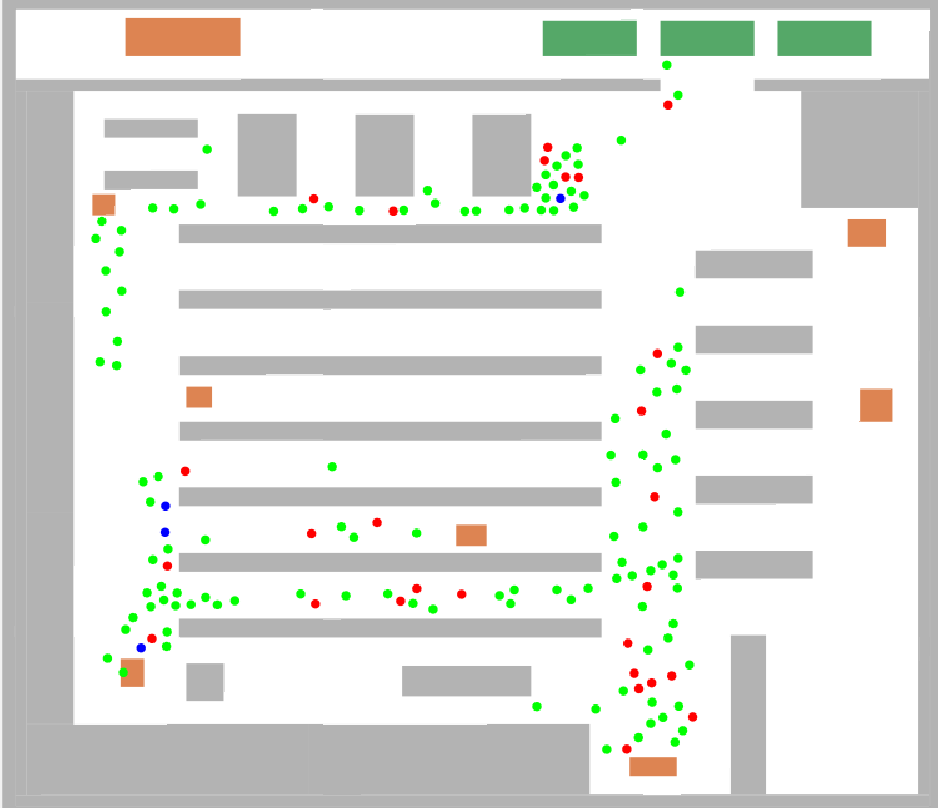
\includegraphics[width=\textwidth]{images/task5_shoppingmid.png}
        \caption{ Pedestrians are walking around the supermarket}
        \label{fig:supermarket_c}
    \end{subfigure}
    \hfill
    \begin{subfigure}[b]{0.49\textwidth}
        \centering
        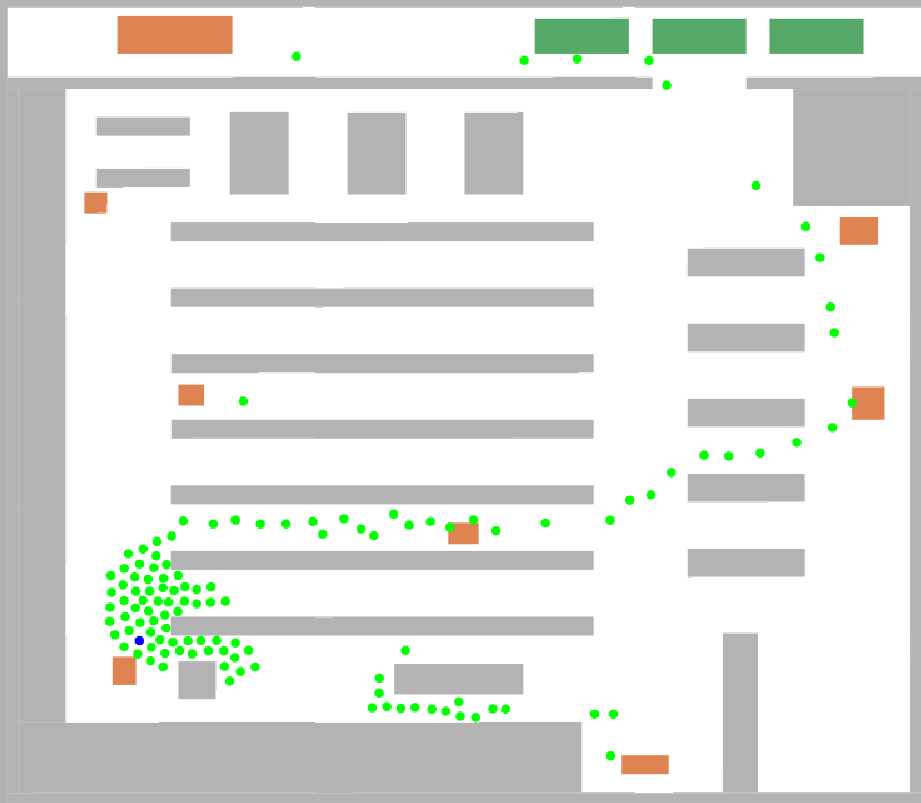
\includegraphics[width=\textwidth]{images/task5_shoppingend.png}
        \caption{Some pedestrians are returning however, some of them are stuck inside of a crowd}
        \label{fig:supermarket_d}
    \end{subfigure}
\caption{Supermarket Scenario for $\texttt{pedPotentialPersonalSpaceWidth} = 0.5$ }
    
\end{figure}

To get pedestrians to take different paths, 3 sources of 50 pedestrians have been implemented (150 in total for the scenarios), each group having different target orders (routings) inside the supermarket before leaving. 
For all the scenarios, the following parameters are fixed and set:
\begin{itemize}
    \item \texttt{infectionsAtStart} : 10 
    \item \texttt{infectionRate} : 0.1
    \item \texttt{infectionMaxDistance} : 1.0
    \item \texttt{recoveredfixedRate} : 0.05
\end{itemize}

To see what happens when increasing the \texttt{pedPotentialPersonalSpaceWidth}, 4 tests have been implemented with different values for this parameter: 0.5, 1.5, 2.5, and 3.5. 

Regarding the paths of the pedestrians, we notice the following during the scenarios: the lower the value of \texttt{pedPotentialPersonalSpaceWidth} is, the more they get stuck in the corridors as different pedestrians headed in different directions hinder each other's motion. Some pedestrians even cannot complete their objective in a time frame of 500 seconds.\\

Regarding the spread of the infection, referring to the SIR visualisations, 
both 0.5 (see figure \ref{fig:t5-s1}) and 1.5 (see figure \ref{fig:t5-s2}) meters produce a high initial spike in infections, in which it subsides faster for a value of 1.5. While there is a difference in the total number of infections, it is a rather small amount. Adding another meter to achieve a \texttt{pedPotentialPersonalSpaceWidth} of 2.5 results in a drastic difference, however, as can be seen in figure \ref{fig:t5-s3}. The initial infection spike is less than 50, and the line of susceptible and removed pedestrians does not intersect, i.e. less than half of the supermarket visitors become infected. Figure \ref{fig:t5-s4} shows an interesting result: The graph does not show even fewer infections like it was to be expected. Despite the efforts to increase the distance between pedestrians, the limited space, particularly at the entrance, leads to crowded conditions, facilitating the transmission of infections. \\

To reduce the number of infections, we want to introduce several ideas: First of all, only a specified amount of pedestrians should be allowed inside a supermarket depending on its size. We made calculations for what could be the best number of people for $\texttt{pedPotentialPersonalSpaceWidth} = 3.5$. It can be seen from figure \ref{fig:graph119}, that when \textbf{119} people were allowed to enter the supermarket, less than 50\% of the people got infected due to a smaller crowd at the entrance.

%will put pitcure
\begin{figure}[H]
    \centering
    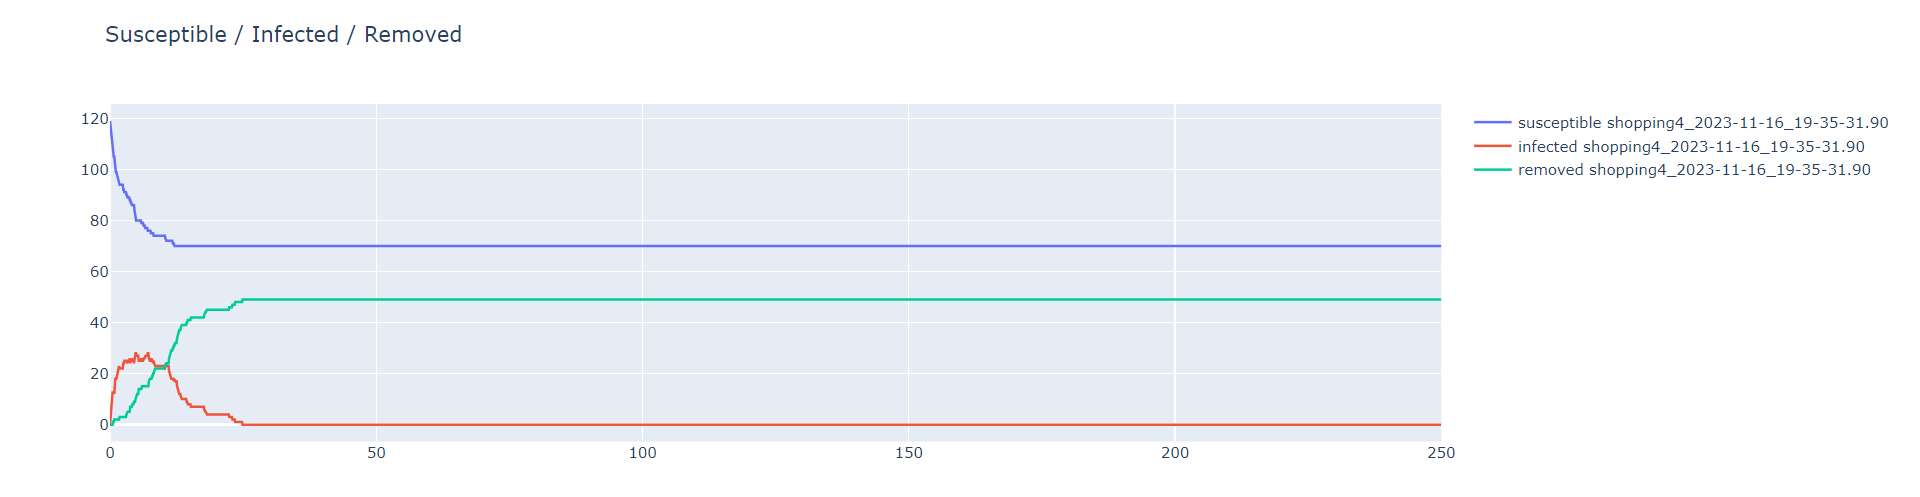
\includegraphics[width=\linewidth]{images/task5_shopping5.png}
    \caption{119 people are allowed to enter the supermarket}
    \label{fig:graph119}
\end{figure}



While waiting outside, the people need to retain distance as well. This can be realized using drawn-on lines in the parking lot as well as using shopping carts for more flexible queues. Both of these methods have been used during the height of the COVID-19 pandemic. \cite{covid-queue-bbc, covoid-queue-wired}


Additionally, specific routes can be marked inside the supermarket to achieve 'one-way streets' to avoid the need to close the gap between pedestrians even for a short amount of time. 


%\begin{center}
\begin{figure}[H]
    \centering
    \begin{subfigure}[t]{\textwidth}
        \centering
        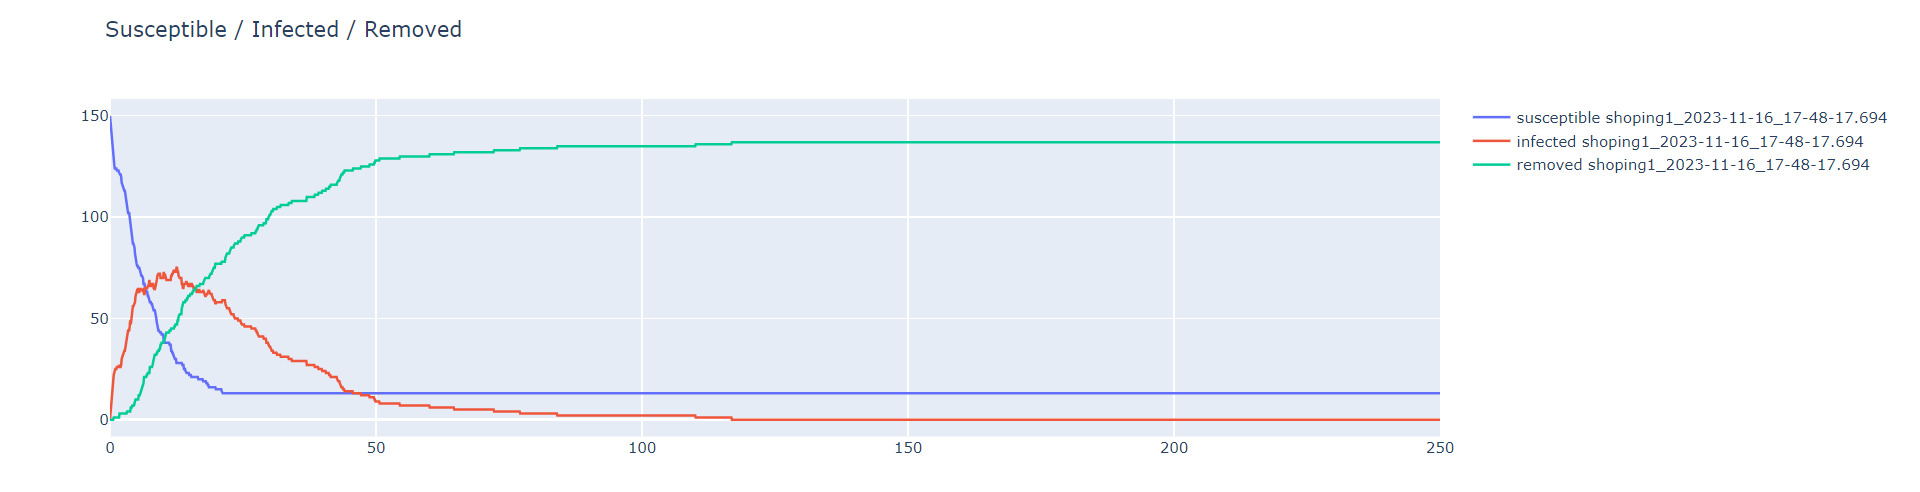
\includegraphics[width=\linewidth]{images/task5_shopping1.png}
        \caption{\texttt{pedPotentialPersonalSpaceWidth} = 0.5}
        \label{fig:t5-s1}
    \end{subfigure}%

    \begin{subfigure}[t]{\textwidth}
        \centering
        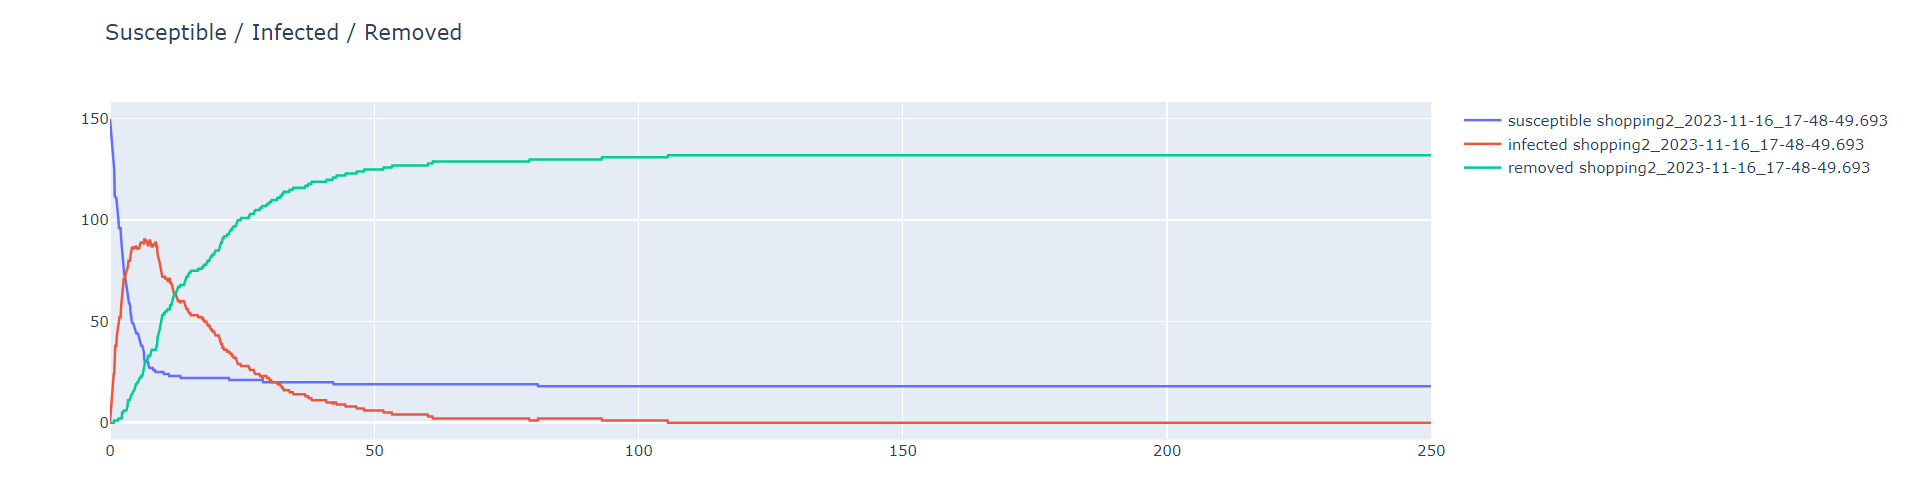
\includegraphics[width=\linewidth]{images/task5_shopping2.png}
        \caption{\texttt{pedPotentialPersonalSpaceWidth} = 1.5}
        \label{fig:t5-s2}
    \end{subfigure}

    \centering
    \begin{subfigure}[t]{\textwidth}
        \centering
        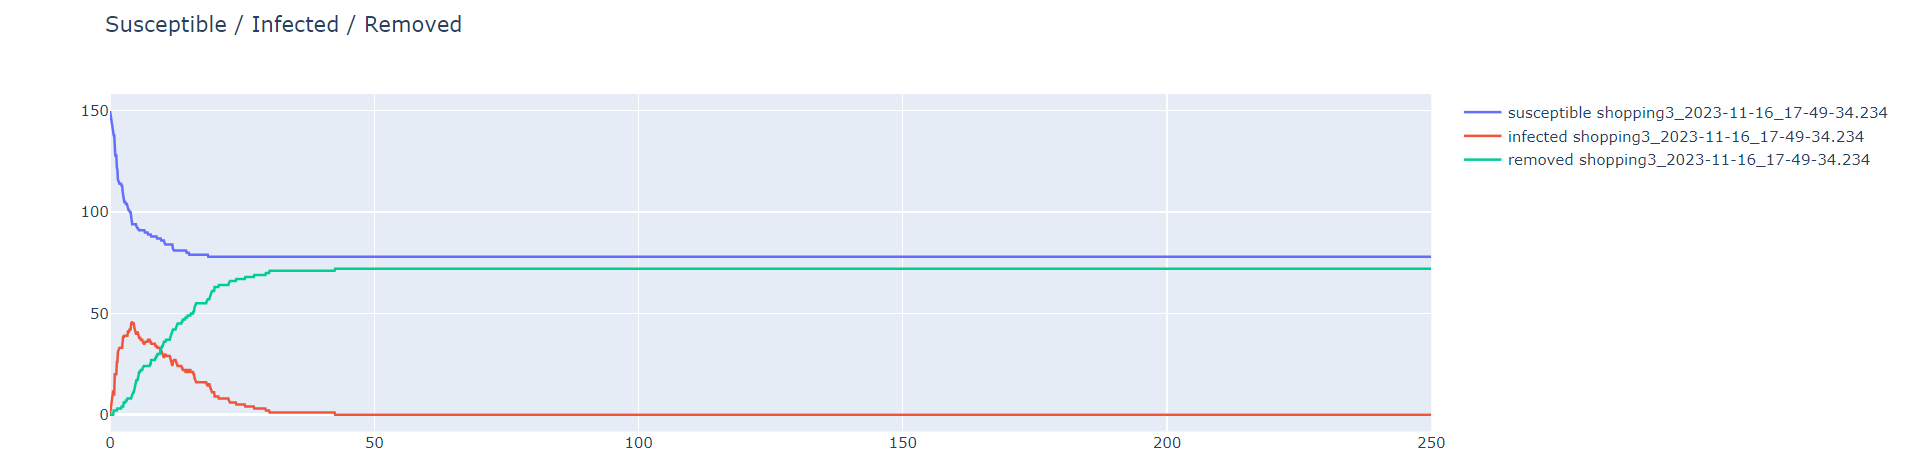
\includegraphics[width=\linewidth]{images/task5_shopping3.png}
        \caption{ \texttt{pedPotentialPersonalSpaceWidth} = 2.5}
        \label{fig:t5-s3}
    \end{subfigure}%
    
    \begin{subfigure}[t]{\textwidth}
        \centering
        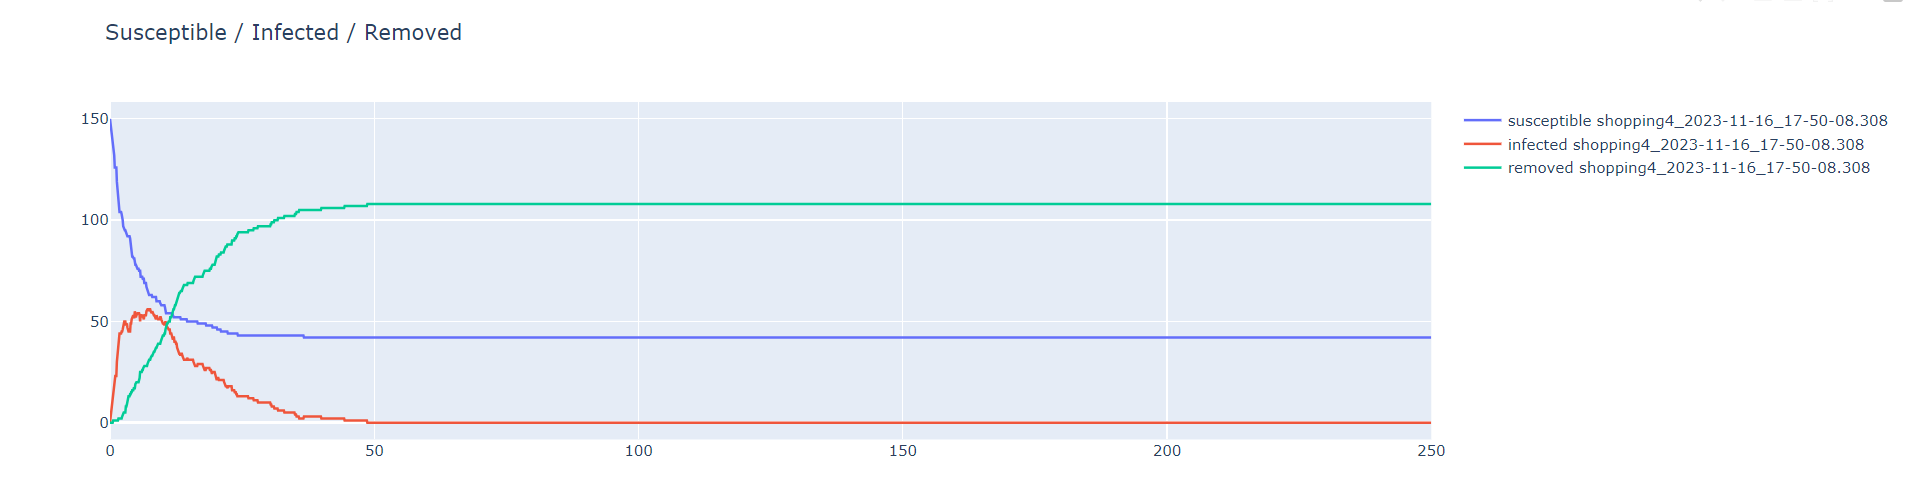
\includegraphics[width=\linewidth]{images/task5_shopping4.png}
        \caption{\texttt{pedPotentialPersonalSpaceWidth} = 3.5}
        \label{fig:t5-s4}
    \end{subfigure}

    \caption{Comparison of different \texttt{pedPotentialPersonalSpaceWidth} in market scenario}
\end{figure}